% !TeX encoding = UTF-8
% !TeX program = XeLaTeX
% !TeX spellcheck = en_US

% Author : Shlw
% Description : TikZ Assignment
\documentclass{standalone}

\usepackage{tikz}

\usetikzlibrary{automata}

\begin{document}

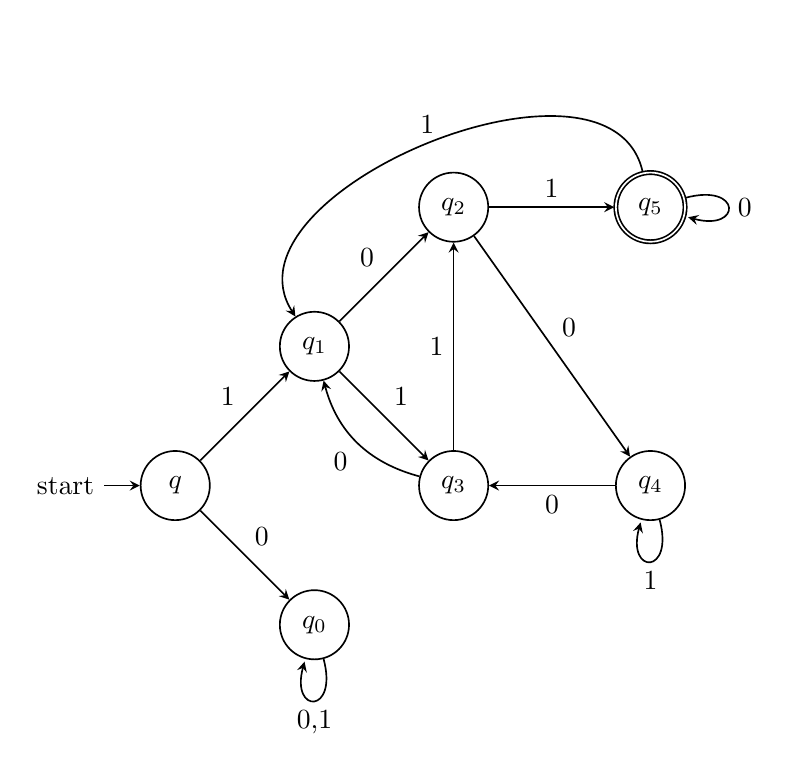
\begin{tikzpicture}[>=stealth,semithick,node distance=2.5cm,auto]
\node[state,initial] (q) {$q$};
\node[state] (q_0) [below right of=q] {$q_0$};
\node[state] (q_1) [above right of=q] {$q_1$};
\node[state] (q_2) [above right of=q_1] {$q_2$};
\node[state,accepting] (q_5) [right of=q_2] {$q_5$};
\node[state] (q_3) [below right of=q_1] {$q_3$};
\node[state] (q_4) [right of=q_3] {$q_4$};

\path[->] (q) edge node {0} (q_0) edge node {1} (q_1)
(q_0) edge [loop below] node {0,1} ()
(q_1) edge node {0} (q_2) edge node {1} (q_3)
(q_2) edge node {1} (q_5) edge node {0} (q_4)
(q_3) edge [bend left] node {0} (q_1) edge node {1} (q_2)
(q_4) edge node {0} (q_3) edge [loop below] node {1} ()
(q_5) edge [loop right] node {0} () edge [bend right=100] node [above] {1} (q_1);
\end{tikzpicture}

\end{document}
